\documentclass[11pt]{article}
\usepackage[margin=2.5cm]{geometry}
\usepackage{amsmath,amssymb}
\usepackage{graphicx}
\usepackage{booktabs}
\usepackage{pgfplots}
\pgfplotsset{compat=1.18}
\usepackage[numbers]{natbib}
\usepackage{hyperref}

% Your own commands. The math preview in Scriptorium knows them too.
\newcommand{\R}{\mathbb{R}}
\newcommand{\E}{\mathbb{E}}

\title{A Short Paper Written in Scriptorium}
\author{Your Name\\\small Your Institution}
\date{\today}

\begin{document}
\maketitle

\begin{abstract}
This template is a starting point for a paper. Replace the text with your own. Along the way it shows what the
editor can do: compile with Ctrl+S, jump between the PDF and the source, complete references and citations, and
preview equations while you type.
\end{abstract}

\section{Introduction}
\label{sec:intro}

Each section of this paper lives in its own file in the \texttt{sections} folder, and \texttt{main.tex} reads them
with \verb|\input|. The outline on the left shows every section of every file, numbered as in the PDF, with its word
count.

Double-click anywhere in the PDF to jump to the line that made it. Press Ctrl+J to see where the cursor is in the
PDF. Hover a citation such as \citet{knuth1984texbook} to see the entry, or a reference such as
Section~\ref{sec:method} to see what it points at. Ctrl+click follows it.

Type \verb|\cite{| and the editor offers the entries of \texttt{references.bib}. Type \verb|\ref{| and it offers
your labels. To add a reference, open the command palette (Ctrl+Shift+P) and choose \emph{Add a reference from a DOI
or arXiv ID}. Classic introductions to the language are \citet{lamport1994latex} and \citet{mittelbach2004companion}.

\section{Method}
\label{sec:method}

Put the cursor inside an equation and the editor shows it rendered, above the line you are typing. It also knows the
commands defined in the preamble, such as \verb|\R| and \verb|\E|. For a state $x \in \R^n$ we minimise
\begin{equation}
  J(\theta) = \E_{x \sim p}\!\left[ \tfrac{1}{2} \lVert f_\theta(x) - y \rVert^2 \right]
            + \lambda \sum_{i=1}^{n} \theta_i^2 ,
  \label{eq:loss}
\end{equation}
where $\lambda > 0$ weighs the regulariser. Equation~\eqref{eq:loss} is a plain least-squares loss. The \emph{Symbols}
panel on the left inserts Greek letters, operators and matrices with a click.

\subsection{Writing tips}

Type \verb|\begin{| to pick an environment: the editor writes the \verb|\end| for you and puts the cursor inside.
Paste an image from the clipboard, or drop one on the editor, and it is saved in a figures folder with a figure
around it.

\section{Results}
\label{sec:results}

Figure~\ref{fig:curve} is drawn by \texttt{figures/curve.tex} with pgfplots, so it needs no image file.
Table~\ref{tab:results} uses the booktabs rules, which the \emph{Insert a table} command also uses.

\begin{figure}[t]
  \centering
  % A plot drawn by pgfplots: no image file needed.
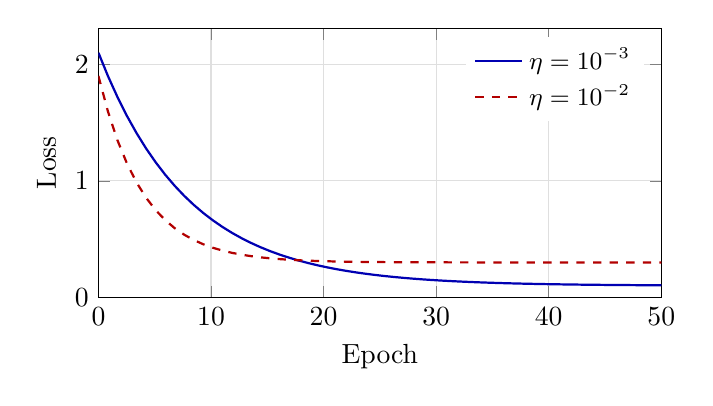
\begin{tikzpicture}
  \begin{axis}[
      width=0.72\linewidth, height=5cm,
      xlabel={Epoch}, ylabel={Loss},
      xmin=0, xmax=50, ymin=0,
      legend pos=north east, legend style={draw=none, font=\small},
      grid=major, grid style={gray!25},
    ]
    \addplot[thick, blue!70!black, domain=0:50, samples=60] {0.1 + 2*exp(-x/8)};
    \addlegendentry{$\eta = 10^{-3}$}
    \addplot[thick, red!70!black, dashed, domain=0:50, samples=60] {0.3 + 1.6*exp(-x/4)};
    \addlegendentry{$\eta = 10^{-2}$}
  \end{axis}
\end{tikzpicture}

  \caption{Training loss for two learning rates.}
  \label{fig:curve}
\end{figure}

\begin{table}[t]
  \centering
  \caption{Final loss and training time.}
  \label{tab:results}
  \begin{tabular}{lcc}
    \toprule
    Learning rate & Final loss & Time (min) \\
    \midrule
    $10^{-3}$ & 0.12 & 14 \\
    $10^{-2}$ & 0.31 & 9 \\
    \bottomrule
  \end{tabular}
\end{table}

When the paper is done, the download button above the PDF saves it, and the \emph{Changes} panel commits your work
if the folder is in git.


\bibliographystyle{plainnat}
\bibliography{references}

\end{document}
